\let\negmedspace\undefined
\let\negthickspace\undefined
\documentclass[journal]{IEEEtran}
\usepackage[a5paper, margin=10mm, onecolumn]{geometry}
%\usepackage{lmodern} % Ensure lmodern is loaded for pdflatex
\usepackage{tfrupee} % Include tfrupee package

\setlength{\headheight}{1cm} % Set the height of the header box
\setlength{\headsep}{0mm}     % Set the distance between the header box and the top of the text

\usepackage{gvv-book}
\usepackage{gvv}
\usepackage{cite}
\usepackage{amsmath,amssymb,amsfonts,amsthm}
\usepackage{algorithmic}
\usepackage{graphicx}
\usepackage{textcomp}
\usepackage{xcolor}
\usepackage{txfonts}
\usepackage{listings}
\usepackage{enumitem}
\usepackage{mathtools}
\usepackage{gensymb}
\usepackage{comment}
\usepackage[breaklinks=true]{hyperref}
\usepackage{tkz-euclide} 
\usepackage{listings}
% \usepackage{gvv}                                        
\def\inputGnumericTable{}                                 
\usepackage[latin1]{inputenc}                                
\usepackage{color}                                            
\usepackage{array}                                            
\usepackage{longtable}                                       
\usepackage{calc}                                             
\usepackage{multirow}                                         
\usepackage{hhline}                                           
\usepackage{ifthen}                                           
\usepackage{lscape}
\usepackage{xparse}
\begin{document}

\bibliographystyle{IEEEtran}
\vspace{3cm}

\title{1.1.7.2}
\author{EE24BTECH11039 - Mandala Ranjith
}
% \maketitle
% \newpage
% \bigskip
{\let\newpage\relax\maketitle}

\renewcommand{\thefigure}{\theenumi}
\renewcommand{\thetable}{\theenumi}
\setlength{\intextsep}{10pt} % Space between text and floats


\numberwithin{equation}{enumi}
\numberwithin{figure}{enumi}
\renewcommand{\thetable}{\theenumi}


\textbf{Question}:x\\
The points $\brak{1,2}$ , $\brak{0,0}$ and $\brak{a,6}$ are collinear
\\ \textbf{Solution: }\\
    \begin{table}[h!]    
      \centering
      
\begin{tabular}{|m{5em} |m{10em}| m{10em} | }
\hline
\textbf{Symbol} & \textbf{Value} & \textbf{Description} \\
\hline 
\textbf{A} & $\myvec{4\\3}$ & Point \textbf{A} \\
\hline 
\textbf{B} & $\myvec{0\\0}$ & Point \textbf{B} \\
\hline
\textbf{C} & $\myvec{a\\6}$ & Point \textbf{C} \\
\hline
\textbf{M} & $\myvec{\textbf{A} - \textbf{B} & \textbf{C} - \textbf{B}}$ & \\
\hline
\end{tabular}


      \caption{}
    \end{table}\\
    Performing row operation on $\vec{M}$ \\
\begin{align}
	\textbf{M'} &=  \myvec{1 & a\\0 & 6-2a}
\end{align}
	for $\text{A},\text{B},\textbf{C}$ to be collinear,
\begin{align}
        rank\brak{\vec{M}} & =1\\
	6-2a & =0\\
	a & =3
\end{align}
	
    \begin{figure}[h]
        \centering
       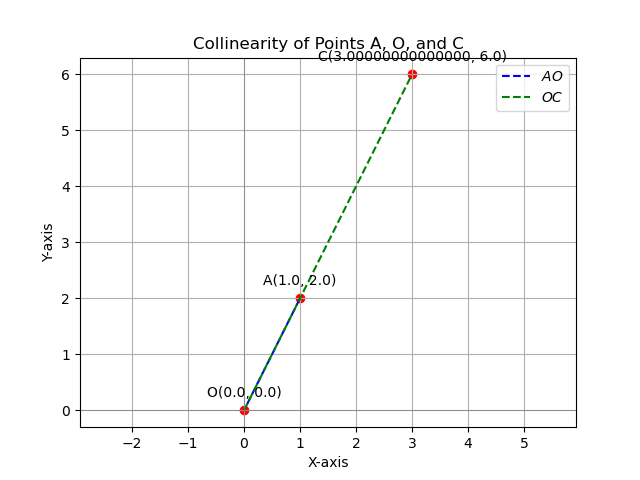
\includegraphics[width=0.7\linewidth]{./figs/fig1.png}
       \caption{}
       \label{graph}
    \end{figure}



\end{document}  


